    \section*{Chapter 12}
    
 \begin{Solution}{12.1}
 
 $\lceil{x}\rceil$ is the smallest integer greater than or equal to $x$.\\[5pt]

\end{Solution}

 \begin{Solution}{12.2}
 \ 
 \vskip 5pt

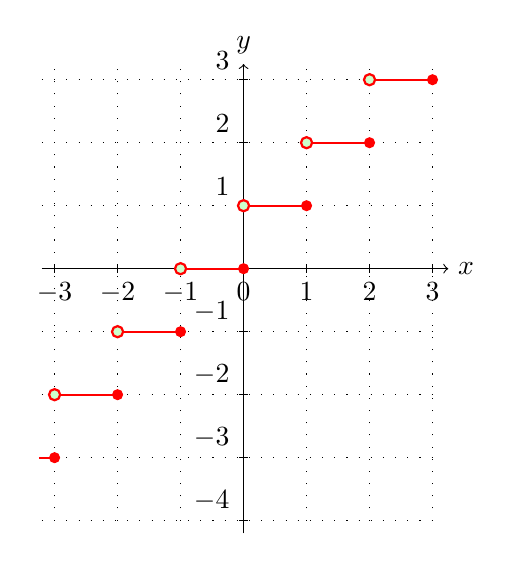
\begin{tikzpicture}[scale=0.80,
  font=\sffamily,
  source/.style={fill,circle,fill=red,inner sep=0.5mm},
  sink/.style={draw,circle,fill=green!20,inner sep=0.5mm},
  every node/.style={align=center}]

%draw axes and grid
    \draw[loosely dotted] (-3.2,-4) grid (3,3.2);
    \draw[->] (-3.2,0) -- (3.25,0) node[right] {$x$};
    \draw[->] (0,-4.2) -- (0,3.25) node[above] {$y$};
   
 %label and tic axes
    \foreach \x/\xtext in {-3/-3, -2/-2,-1/-1,0/0,1/1,2/2, 3/3}
    \draw[shift={(\x,0)}] (0pt,2pt) -- (0pt,-2pt) node[below] {$\xtext$};
    \foreach \y/\ytext in {-4/-4, -3/-3, -2/-2, -1/-1, 1/1, 2/2, 3/3}
    \draw[shift={(0,\y)}] (2pt,0pt) -- (-2pt,0pt) node[above left] {$\ytext$};

%draw jumps
  \foreach \x in {-3,-2,...,2} {
%     \draw[red,thick,dashed]  (\x,\x+1) node[sink] {} -- (\x+1,\x+1) node[source] {};
    \draw[red,thick]  (\x,\x+1) node[sink] {} -- (\x+1,\x+1) node[source] {}; }
%draw a partial jump
    \draw[red,thick]  (-3.25,-3.00) node {} -- (-3.00,-3.00) node[source] {};
   

    \end{tikzpicture}\\[5pt]


\end{Solution}

\begin{Solution}{12.3}
\
\vskip 5pt
We could fall back on the classic {\itshape plot{-}a{-}billion{-}points} method of graphing,
but it is a better idea to think first. The graph ought to look a lot like the graph of $y = \lfloor{x}\rfloor$,
but the jumps will move to new spots. In particular, there will be a jump up by $1$  whenever $x$ reaches a value 
where $2x-1 = n$,
for $n$ equal an integer. In other words, there will be jumps when $x= \frac{n+1}{2}$ for integers $n$.

So the graph will show jumps at 
\[
\ldots, - 2=\frac{-4}{2}, \frac{-3}{2}, -1 = \frac{-2}{2}, \frac{-1}{2}, 0 = \frac{0}{2}, \frac{1}{2}, 1\frac{2}{2}, \frac{3}{2}, \ldots, \frac{4}{2}.
\]
Moreover, for the integer $n$, the jump at $x=\frac{n+1}{2}$ will be from $n-1$ to $n$. That's enough to draw the graph:
it looks exactly like the graph of $y = \lfloor{x}\rfloor$, except jumps come at multiples of $\frac{1}{2}$ instead of at the integers.
That makes the graph easy to draw since we can {\itshape cheat} by dividing all the integer marks on the $x${-}axis by $2$ in the graph of $y = \lfloor {x}\rfloor$.  

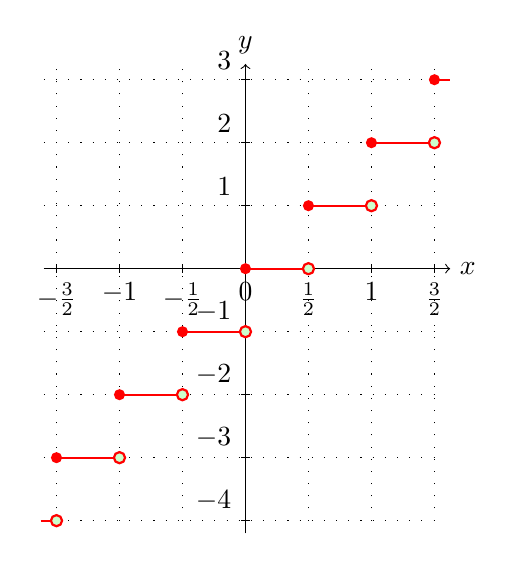
\begin{tikzpicture}[scale=0.80,
  font=\sffamily,
  source/.style={fill,circle,fill=red,inner sep=0.5mm},
  sink/.style={draw,circle,fill=green!20,inner sep=0.5mm},
  every node/.style={align=center}]

%draw axes and grid
    \draw[loosely dotted] (-3.2,-4) grid (3,3.2);
    \draw[->] (-3.2,0) -- (3.25,0) node[right] {$x$};
    \draw[->] (0,-4.2) -- (0,3.25) node[above] {$y$};
   
 %label and tic axes
    \foreach \x/\xtext in {-3/-\frac{3}{2}, -2/-1,-1/-\frac{1}{2},0/0,1/\frac{1}{2},2/1, 3/\frac{3}{2}}
    \draw[shift={(\x,0)}] (0pt,2pt) -- (0pt,-2pt) node[below] {$\xtext$};
    \foreach \y/\ytext in {-4/-4, -3/-3, -2/-2, -1/-1, 1/1, 2/2, 3/3}
    \draw[shift={(0,\y)}] (2pt,0pt) -- (-2pt,0pt) node[above left] {$\ytext$};

%draw jumps
  \foreach \x in {-3,-2,...,2} {
%     \draw[red,thick,dashed]  (\x,\x) node[sink] {} -- (\x,\x+1) node[source] {};
    \draw[red,thick]  (\x,\x) node[source] {} -- (\x+1,\x) node[sink] {}; }
%draw partial jumps
    \draw[red,thick]  (-3.25,-4.00) node {} -- (-3.00,-4.00) node[sink] {};
    \draw[red,thick]  (3.00,3.00) node[source] {} -- (3.25,3.00) node {};

    \end{tikzpicture}\\[5pt]


\end{Solution}

 \begin{Solution}{12.4}
 
 Thinking: the graph of $y =\lfloor{x-1}\rfloor$ will look just like the graph of $y=\lfloor{x}\rfloor$
 shifted one unit the the right, and the factor of $2$ in $y = 2\lfloor{x-1}\rfloor$ will move each
 horizontal segment of the graph to twice its original distance from the $x${-}axis. Put those 
 two pieces together:
 \begin{tikzpicture}[scale=0.80,
  font=\sffamily,
  source/.style={fill,circle,fill=red,inner sep=0.5mm},
  sink/.style={draw,circle,fill=green!20,inner sep=0.5mm},
  every node/.style={align=center}]

%draw axes and grid
    \draw[loosely dotted] (-3.2,-4) grid (3,3.2);
    \draw[->] (-3.2,0) -- (3.25,0) node[right] {$x$};
    \draw[->] (0,-4.2) -- (0,3.25) node[above] {$y$};
   
 %label and tic axes
    \foreach \x/\xtext in {-3/-3, -2/-2,-1/-1,0/0,1/1,2/2, 3/3}
    \draw[shift={(\x,0)}] (0pt,2pt) -- (0pt,-2pt) node[below] {$\xtext$};
    \foreach \y/\ytext in {-4/-8, -3/-6, -2/-4, -1/-2, 1/2, 2/4, 3/6}
    \draw[shift={(0,\y)}] (2pt,0pt) -- (-2pt,0pt) node[above left] {$\ytext$};

%draw jumps
  \foreach \x in {-3,-2,...,2} {
%     \draw[red,thick,dashed]  (\x,\x) node[sink] {} -- (\x,\x+1) node[source] {};
    \draw[red,thick]  (\x+1,\x) node[source] {} -- (\x+2,\x) node[sink] {}; }
%draw partial jumps
%    \draw[red,thick]  (-3.25,-4.00) node {} -- (-3.00,-4.00) node[sink] {};
%    \draw[red,thick]  (3.00,3.00) node[source] {} -- (3.25,3.00) node {};

    \end{tikzpicture}\\[5pt]

\end{Solution}

\begin{Solution}{12.5}
The functons $f(x) = 18$ and $g(x) = \frac{x^{3}}{2}$ cross when $18x = \frac{x^{3}}{2}$. That
is, when 
\begin{align*}
36x &= x^{3}\\
x^{3} - 36x &= 0\\
x(x^{2}- 36) &= 0\\
x(x-6)(x+6) &= 0\\
x &= -6, 0, 6\\
\end{align*}
as seen in the graph.

So, for $x>0$,  $g$ catches $f$ at $x = 6$ for $x>0$. 

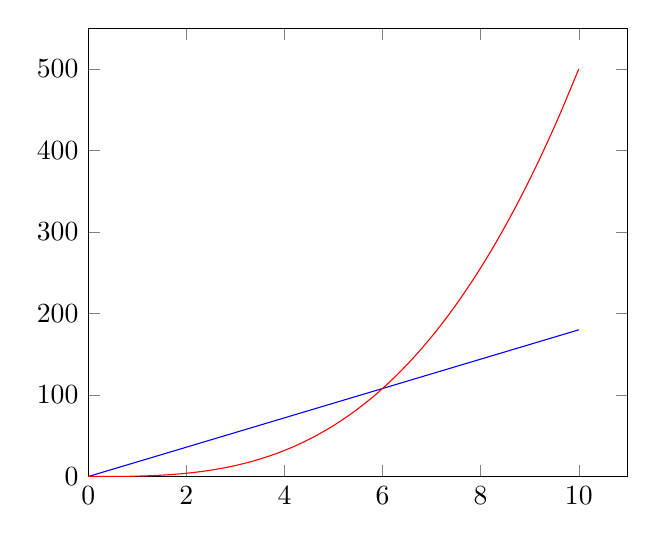
\begin{tikzpicture}
\begin{axis}[scaled ticks=false,xmin=0,ymin=0]
\addplot[domain=0:10, blue, smooth] {18*x};
\addplot[domain=0:10, red, smooth] {x*x*x/2};
\end{axis}
\end{tikzpicture}
\end{Solution}

\begin{Solution}{12.6}


The exponential function $g(x) = 2^x$ ultimately beats the power function $f(x) = 4x^5$. 
To show that, lets find a number $x>1$ so that
$\ln(2^x) > \ln(4x^5)$.   That inequality can be rewritten as $x\ln{2} > \ln{4} + 5\ln{x}$.
Since all we care about is showing there is an $x$ for which that inequality is true, we can 
make some simplifying substitutions:  if $\frac{x}{2} > 2 +5\ln{x}$, that would be guarantee 
$x\ln{2} > \ln{4} + 5\ln{x}$. So let's see if we can find $x$ so that $x > 4 + 10\ln{x}$, and since
we can make $x$ as large as we want, we can also guarantee $\ln{x}\geq 4$. Consequently
we need only be sure we can pick $x$ with $x > 11\ln{x}$. Thinking about the graphs of
$y = x$ and $y = 11 \ln{x}$, we can see there will certainly be such an $x$.  If we know a bit 
of calculus, we can compute slopes of tangent lines to the two curves to show there is such an $x$.
If we have a computer algebra system, we can find a specific value of such an $x$. In fact, 
it turns out that $41$ is the smallest integer greater than $1$ for which $x > 11\ln{x}$. \\[5pt]


\end{Solution}

\begin{Solution}{12.7}

Assuming the other buttons are in working order, we can use the fact that $\log(2^{\sqrt{2}})= (\sqrt{2})\log{2}$.
Here are the steps:
\begin{itemize}
\item get square root of $2$ (result: $1.41421\cdots$)\\
\item multiply by $\log{2}$ (result: $.42572\cdots$)\\
\item take inverse log ($10^x$ button for if you are \\
using base $10$ logs) (result $2.66514\cdots = 2^{\sqrt{2}}$).\\[5pt]
\end{itemize}

\end{Solution} 